\index{general}{$P_1^+\times P_0$}
\begin{flushright} {\tiny {\color{gray} \tt pair\_p1pp0.tex}} \end{flushright}
%~~~~~~~~~~~~~~~~~~~~~~~~~~~~~~~~~~~~~~~~~~~~~~~~~~~~~~~~~~~~~~~~~~~~~~~~~~~~~~~~~~~~~~~~~~~~~~~~~~

\begin{center}
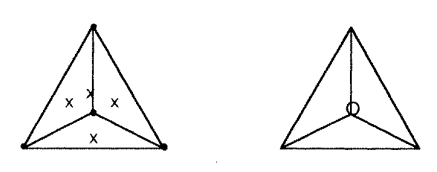
\includegraphics[width=6cm]{images/pair_p1pp0/p1pp0}\\
{\captionfont Taken from \textcite{begt92} (1992).}
\end{center}

In Table I of \textcite{begt92} (1992) we find:
\begin{eqnarray}
\bN_1(r,s,t) &=& (1-r-s-t)-\frac13 (\bN_5+\bN_6+\bN_7) \qquad \vec{r}_1=(0,0,0) \nn\\
\bN_2(r,s,t) &=& r-\frac13 (\bN_5+\bN_6+\bN_8)         \qquad \vec{r}_2=(1,0,0) \nn\\
\bN_3(r,s,t) &=& s-\frac13 (\bN_5+\bN_7+\bN_8)         \qquad \vec{r}_3=(0,1,0) \nn\\
\bN_4(r,s,t) &=& t-\frac13 (\bN_6+\bN_7+\bN_8)         \qquad \vec{r}_4=(0,0,1) \nn\\
\bN_5(r,s,t) &=& 27(1-r-s-t)rs          \qquad \vec{r}_5=(\frac13,\frac13,0) \nn\\
\bN_6(r,s,t) &=& 27(1-r-s-t)rt          \qquad \vec{r}_6=(\frac13,0,\frac13) \nn\\
\bN_7(r,s,t) &=& 27(1-r-s-t)st          \qquad \vec{r}_7=(0,\frac13,\frac13) \nn\\
\bN_8(r,s,t) &=& 27rst  \qquad\qquad\qquad\quad \vec{r}_8=(\frac13,\frac13,\frac13) 
\end{eqnarray}
Note that we can verify that
\begin{eqnarray}
\sum_{i=1}^8 \bN_i(r,s,t) 
&=& \bN_1 +\bN_2 +\bN_3 +\bN_4 +\bN_5 +\bN_6 +\bN_7 +\bN_8 \nn\\
&=& (1-r-s-t)-\frac13 (\bN_5+\bN_6+\bN7) \nn\\
&+& r-\frac13 (\bN_5+\bN_6+\bN8)  
 +  s-\frac13 (\bN_5+\bN_7+\bN8) 
 +  t-\frac13 (\bN_6+\bN_7+\bN8) \nn\\
&+& \bN_5 + \bN_6 + \bN_7 + \bN_8  \nn\\
&=& 1
+(-\frac13 -\frac13 -\frac13+1)\bN_5
+(-\frac13 -\frac13 -\frac13+1)\bN_6
+(-\frac13 -\frac13 -\frac13+1)\bN_7
+(-\frac13 -\frac13 -\frac13+1)\bN_8 \nn\\
&=& 1
\end{eqnarray}



